\documentclass[11pt,a4paper]{article}

\usepackage[margin=1.05in]{geometry}
\usepackage{amsmath,amssymb,amsthm}
\usepackage{graphicx}
\usepackage{mathtools}
\usepackage{stmaryrd}
\usepackage{booktabs}
\usepackage{listings}
\usepackage{xcolor}
\usepackage{tikz}
\usetikzlibrary{arrows.meta}
\usepackage[colorlinks=true,linkcolor=black,citecolor=black,urlcolor=blue]{hyperref}
\usepackage{enumitem}
\usepackage[T1]{fontenc}
\usepackage[protrusion=true,expansion=false]{microtype}
\setlength{\emergencystretch}{2.5em}

%%%%%%%%%%%%%%%%%%%%%%%%%%%%%%%%%%%%%%%%%%%%%%%%%%%%%%%%%%%%%%%%%%%%%%%%%%%%%%%
% Theorem environments
%%%%%%%%%%%%%%%%%%%%%%%%%%%%%%%%%%%%%%%%%%%%%%%%%%%%%%%%%%%%%%%%%%%%%%%%%%%%%%%
\theoremstyle{plain}
\newtheorem{theorem}{Theorem}[section]
\newtheorem{proposition}[theorem]{Proposition}
\newtheorem{lemma}[theorem]{Lemma}
\newtheorem{corollary}[theorem]{Corollary}
\newtheorem{conjecture}[theorem]{Conjecture}

\theoremstyle{definition}
\newtheorem{definition}[theorem]{Definition}
\newtheorem{example}[theorem]{Example}
\newtheorem{principle}[theorem]{Principle}
\newtheorem{obligation}[theorem]{Obligation}
\newtheorem{finding}[theorem]{Empirical finding}

\theoremstyle{remark}
\newtheorem{remark}[theorem]{Remark}

%%%%%%%%%%%%%%%%%%%%%%%%%%%%%%%%%%%%%%%%%%%%%%%%%%%%%%%%%%%%%%%%%%%%%%%%%%%%%%%
% Macros.  NOTATION RULES OBSERVED THROUGHOUT:
%   * the rho calculus is never written with the Greek letter rho
%   * quoting is @P, dropping is *x; corner quotes are pre-2016 notation
%%%%%%%%%%%%%%%%%%%%%%%%%%%%%%%%%%%%%%%%%%%%%%%%%%%%%%%%%%%%%%%%%%%%%%%%%%%%%%%
\newcommand{\rhoc}{\textsf{rho}}
\newcommand{\grho}{\textsf{rho}_{\V}}
\newcommand{\sem}[1]{[\![#1]\!]}
\newcommand{\V}{\mathbb{V}}
\newcommand{\Bool}{\mathbb{B}}
\newcommand{\Rnn}{\mathbb{R}_{\geq 0}}
\newcommand{\Cx}{\mathbb{C}}
\newcommand{\Nat}{\mathbb{N}}
\newcommand{\Reals}{\mathbb{R}}
\newcommand{\Proc}{\mathcal{P}}
\newcommand{\Names}{\mathcal{N}}
\newcommand{\Reach}{\mathrm{Reach}}
\newcommand{\supp}{\mathrm{supp}}
\newcommand{\scong}{\equiv}
\newcommand{\tensorv}{\otimes}
\newcommand{\sumv}{\oplus}
\newcommand{\Cand}{\mathrm{Cand}}
\newcommand{\Out}{\mathrm{out}}
\newcommand{\crisp}[1]{\lceil #1 \rceil}
\newcommand{\pow}{\mathrm{pow}}
\newcommand{\str}{\mathrm{s}}
\newcommand{\conf}{\mathrm{c}}
\newcommand{\ev}{\mathrm{n}}
\newcommand{\Fish}{\mathcal{I}}
\newcommand{\Score}{\mathcal{S}}
\newcommand{\lolli}{\mathrel{\reflectbox{$\multimap$}}}

\lstdefinestyle{rholang}{
  basicstyle=\ttfamily\small,
  keywordstyle=\bfseries,
  morekeywords={for,new,in,where,contract,match,if,else},
  columns=fullflexible,
  keepspaces=true,
  showstringspaces=false,
  breaklines=true,
  frame=single,
  framesep=5pt,
  rulecolor=\color{black!35},
  xleftmargin=6pt,
  aboveskip=9pt,
  belowskip=9pt
}
\lstset{style=rholang}

%%%%%%%%%%%%%%%%%%%%%%%%%%%%%%%%%%%%%%%%%%%%%%%%%%%%%%%%%%%%%%%%%%%%%%%%%%%%%%%

\title{\bfseries Graded Where-Clauses over the Reals\\[4pt]
\large One-dimensional grading as the mortal scientist's gradient,\\
and probabilistic logic as the metric that gradient requires}

\author{L.\,G.\ Meredith\\ \small F1R3FLY.io}

\date{F1R3FLY.io working note --- August 2026\\[2pt]
\normalsize Paper II of three; supersedes the $\Rnn$ half of
\emph{Graded Where-Clauses}}

\begin{document}
\maketitle

\begin{abstract}
The rho calculus does not say how the non-determinism of a race is resolved.
The companion papers treat that silence as a parameter and instantiate it: with
$\V = \Cx$ one obtains amplitudes and the Born rule. Here $\V = \Rnn$, and the
question is not what a program means but what a \emph{learner} can do with a
value it is allowed to tune.

The answer turns on one structural fact. A learner holding a graded hypothesis
has two degrees of freedom, and they live in different geometries. The formulae
form an ultrametric space, in which there is no betweenness and therefore no
gradient; the values form an ordered continuum, in which there is nothing but
gradient. So the hypothesis space is a fibration, and one-dimensional grading is
exactly the enrichment that makes the fibre navigable.

We make the fibre gradient precise. Over $\Rnn$ a modality-free clause is a
posynomial in its scalar parameters, hence smooth and log-convex in
log-coordinates; the likelihood of a causal history factors over firing sites;
and the parameter gradient of that likelihood decomposes into a sum of local
scores, each computable at the site from the candidate values the site already
had. Differentiating a \emph{modal} clause is the adjoint of the same transfer
operator whose Neumann series defines the graded fixed point, so
differentiability and existence hold under one condition rather than two. None
of this survives the passage to $\Cx$, which is the structural reason the
learning instance and the quantum instance are separate papers.

The headline result is that the metric on the fibre is not free, and that
choosing it correctly yields probabilistic logic rather than requiring it. The
Euclidean gradient on a strength in $[0,1]$ does not know how much evidence
backs the current value; the natural gradient does, through the Fisher
information, and the Fisher information is a count. Revising a PLN truth value
$(\str,\ev)$ by one observation is \emph{exactly} the natural-gradient step with
unit step size and the metric evaluated at the posterior count --- measured worst
discrepancy $1.110\times10^{-16}$ over $20{,}000$ random instances, against
$4.612\times10^{-1}$ if the metric is taken at the prior count. Because the
metric is evaluated after the increment the step is implicit, hence
unconditionally stable: over $200{,}000$ random steps it never leaves the unit
interval, while the explicit forms are absorbed at the boundary or escape it
outright. Confidence is therefore not a second truth value. It is the metric on
the first.

The consequences are ecological. The confidence schedule satisfies the
Robbins--Monro conditions for every value of PLN's personality parameter $k$, so
$k$ governs the transient and not the limit --- and only a mortal learner can be
harmed by a transient. We measure the optimum for $k$ across the three
distributions that specify an ecology: over trophic types, over inedibles, and
over token reservoirs housed in no computation. Under expected yield and under
log wealth the optima differ systematically and by a factor of seven at the
baseline, and the two criteria disagree not only about the personality but about
whether learning is worth anything at all. Finally, two learners sharing a
belief namespace exhibit the failure the conservation laws predict: evidence is
not conserved, revision presumes independence, and circulating testimony inflates
the count without adding information. In gradient terms the inflated count is a
collapsed step size, so the pathology of minted confidence is not recklessness
but rigidity.
\end{abstract}

\tableofcontents

%==============================================================================
\section{Introduction}\label{sec:intro}

\subsection{Where the choice is}

A rho term may offer several ways to take a step. Two messages waiting on one
channel and a single receipt listening there is the smallest example: either
message may be consumed, the calculus says both are possible, and it says nothing
about which. An implementation must decide, and the decision is not in the
language. In the classical implementation it is made by the physical races of
cores against a tuple space; in the companion paper on the complex instance it is
made by the Born rule.

The design shared by all three papers is one line of grammar. The \texttt{where}
clause of a for-comprehension, which in \rhoc{} 1.4 is a Boolean guard, is
allowed to take values in a commutative semiring $\V$, and is evaluated once per
candidate match rather than once per receipt. When $\V = \Bool$ nothing changes.
When $\V$ is something else, the clause is a weight on a branch, written in the
program, by the programmer, at the point where the branching happens.

This paper takes $\V = \Rnn$.

\subsection{The thesis}\label{ssec:thesis}

The reason to care about $\Rnn$ is not that it gives a stochastic semantics.
Weighted transition systems are old, and a semiring-valued weight on a transition
is not by itself news. The reason to care is that $\Rnn$ is
\emph{one-dimensional and ordered}, and that a learner whose hypotheses are
formulae has, without it, nowhere to put a gradient.

The mortal scientist of the companion programme holds hypotheses drawn from a
logic generated by the term structure of \rhoc{}. Those formulae are metrised by
modal depth: two formulae agreeing to depth $n$ are within $2^{-n}$. That metric
is an ultrametric, and an ultrametric has no betweenness --- for distinct
$\varphi$ and $\psi$ there is no formula standing partway between them in the
sense a convex combination would. A gradient presupposes a direction one may move
along by an arbitrarily small amount. The hypothesis lattice supplies branching
instead, so the only search available on it is tree search, and a theorem of
confinement says an incremental walk never leaves the ball it began in.

Grading changes this, but not by repairing the lattice. It adds a second
coordinate that lives somewhere else:

\begin{quote}\itshape
A graded hypothesis is a pair, a formula and a value. Changing the value is a
move of distance zero in the ultrametric. So the hypothesis space is not a metric
space with a decoration; it is a fibration, with the formula lattice as base and
a $\V$-valued fibre over each point --- and the fibre is where gradient descent
lives.
\end{quote}

That much is stated in the omnibus. What it leaves open is everything a learner
would need in order to act on it. Which gradient? Of what objective? Computed
where, and by whom? Is it available at all when the clause carries a modality?
And, given that a value in $[0,1]$ can be pushed in a direction, what is the
right size of push?

The last question is the one with the interesting answer, and it is the
organising claim of this paper. The naive gradient on a strength is wrong in a
specific and diagnosable way: it does not know how much evidence stands behind
the value it is moving. Correcting it requires a metric on the fibre, the metric
is the Fisher information, the Fisher information for a Bernoulli parameter is an
evidence count, and a strength together with an evidence count is a PLN simple
truth value. Probabilistic logic is not adopted here as an application. It is
what one gets by asking for the gradient to be taken correctly.

\subsection{Contributions}

\begin{enumerate}[leftmargin=1.6em,itemsep=2pt]
\item A definition of the parameters of a graded clause, and the observation that
over $\Rnn$ a modality-free clause is a posynomial in them: smooth everywhere on
the positive orthant, and log-convex in log-coordinates
(\S\ref{sec:gradient}, Proposition~\ref{prop:posy}). Its normalisation is not
log-convex, so the fibre is smooth but not convex; both facts are measured.
\item A decomposition theorem: the parameter gradient of the log-likelihood of a
causal history is the sum of local scores, one per firing site, each computable
from the candidate weights that site already evaluated
(Theorem~\ref{thm:score}). The causal-history quotient of the companion paper is
what makes the statement well posed, and the estimator is exactly the
likelihood-ratio estimator of reinforcement learning, obtained here from the
operational semantics rather than assumed.
\item The modal case, worked. The derivative of a graded fixed point is the
solution of the adjoint system $(\mathrm{Id} - T)\,\partial v = \partial b +
(\partial T) v$, whose Neumann series is the series that defines the fixed point
itself, so differentiability and existence are one condition
(Theorem~\ref{thm:adjoint}).
\item \textbf{The headline.} PLN revision is a natural-gradient step on the
Bernoulli log-likelihood, with unit step size and the Fisher metric evaluated at
the posterior count (Theorem~\ref{thm:natgrad}), and the placement of the metric
after the increment makes the step implicit, hence unconditionally stable
(Corollary~\ref{cor:implicit}). Confidence is the metric, not a second value.
\item The confidence schedule is a Robbins--Monro schedule for every personality
parameter (Proposition~\ref{prop:rm}), so $k$ is a transient parameter, and the
ecology can price what statistics cannot.
\item A robustness study of that price over the three distributions that specify
an ecology --- trophic types, inedibles, and free reservoirs --- reported under
two objectives side by side (\S\ref{sec:robust}).
\item A two-learner testimony experiment showing that circulating belief inflates
the evidence count without adding information, and that the resulting pathology
is loss of plasticity rather than instability (\S\ref{sec:testimony}).
\item A negative result that justifies the split of this line of work into
separate papers: none of the above is available over $\Cx$, because there is no
per-site likelihood to differentiate (Remark~\ref{rem:nocomplex}).
\end{enumerate}

\subsection{What this paper does not do}

It does not propose a new logic; the hypothesis logic is the one generated by the
term structure, taken as given. It does not claim an empirical result about
agents that use probabilistic logic: the ecology of \S\ref{sec:robust} is a
constructed decision problem, and what is reported is the shape of a robustness
surface over it, not a general fact about learners. It does not implement any of
this in a running node. And it does not treat the complex instance, which is
Paper~I, or the resolution algebra in general, which is Paper~III.

%==============================================================================
\section{The calculus}\label{sec:calculus}

The presentation is self-contained. Readers of Paper~I will find
\S\ref{ssec:syntax} and \S\ref{ssec:permatch} familiar, minus the quantum
namespace, which plays no part here.

\subsection{Terms}\label{ssec:syntax}

\begin{definition}[Syntax]\label{def:syntax}
Processes $P$ and names $x$ are given by
\[
\begin{array}{rcl}
P &::=& 0 \;\mid\; x!(P) \;\mid\; \text{for}(\,\vec{y} \leftarrow \vec{x}
  \;\text{where}\; \psi\,)\,P \;\mid\; P \mid P \;\mid\; *x \\[2pt]
x &::=& @P
\end{array}
\]
A receipt $\text{for}(y_1 \leftarrow x_1 \,\&\, \cdots \,\&\, y_m \leftarrow x_m
\;\text{where}\; \psi)P$ is a \emph{join}: it fires only when every one of its
$m$ patterns is matched. The clause $\psi$ is drawn from the graded formula sort
of \S\ref{ssec:sorts} and takes values in $\V$. Writing the clause is optional;
its absence abbreviates $\crisp{\top}$.
\end{definition}

\begin{definition}[Structural congruence]\label{def:cong}
$\scong$ is the least congruence making $(\;\mid\;, 0)$ a commutative monoid and
satisfying $*@P \scong P$ and $@*x = x$.
\end{definition}

\begin{remark}[Receipts are linear]\label{rem:linear}
A receipt is consumed when it fires. The persistent form, written $\Leftarrow$,
survives; it is available but is not the default, and the distinction matters
here for the same reason it matters in Paper~I. Under a persistent receipt the
two-message configuration of \S\ref{ssec:thesis} is not a race at all: both
messages are eventually consumed, the receipt survives either way, and the two
derivations reconverge. It is linearity that makes the surviving message a record
of which branch was taken.
\end{remark}

\begin{definition}[Candidates]\label{def:cand}
Fix a term $P$ and a receipt occurrence $r$ in it with patterns
$y_1,\dots,y_m$ on channels $x_1,\dots,x_m$. A \emph{candidate} at $r$ is an
injective assignment $\sigma$ of the patterns of $r$ to messages resting on the
corresponding channels. $\Cand(P,r)$ denotes the set of candidates. Two
candidates \emph{contend} if they share a message or share a linear receipt; a
\emph{contention set} is a connected component of the contention relation, and it
is the unit at which weights are normalised.
\end{definition}

\subsection{Two sorts of formula}\label{ssec:sorts}

The logic generated by Definition~\ref{def:syntax} has one structural connective
per term former, a name predicate, and one behavioural modality per rewrite rule
together with a choice of redex position. We keep two sorts.

\begin{definition}[Formula sorts]\label{def:sorts}
The \emph{crisp} sort $\beta$ retains the full propositional structure the target
specification supplies, including negation and fixed points where they exist:
\[
\beta ::= \top \;\mid\; \mathrm{out}(n)\beta \;\mid\; \mathrm{in}(n)\beta
      \;\mid\; \beta \mid \beta \;\mid\; @\beta
      \;\mid\; \beta \wedge \beta \;\mid\; \neg\beta
      \;\mid\; \langle K\rangle\beta \;\mid\; \nu X.\beta .
\]
The \emph{graded} sort $\psi$ has no negation, and takes values in $\V$:
\[
\psi ::= \crisp{\beta} \;\mid\; v \;\mid\; \psi \tensorv \psi
      \;\mid\; \psi \sumv \psi \;\mid\; \langle K\rangle_{\V}\psi
      \;\mid\; X \;\mid\; \mu X.\psi \;\mid\; \nu X.\psi ,
\]
where $v$ ranges over constants of $\V$ and fixed-point variables occur
positively and guarded. The embedding $\crisp{-}$ sends a crisp formula to the
multiplicative unit where it holds and to zero where it does not.
\end{definition}

The two sorts divide the labour cleanly: the crisp sort decides \emph{whether} a
candidate is admissible at all, and the graded sort decides \emph{how much}. The
absence of negation on the graded sort is not an oversight. Over a general
semiring there is no canonical complement, and over $\Rnn$ in particular there
are no additive inverses; \S\ref{ssec:adequacy} shows that this absence is
precisely what makes the present instance the learning instance.

\subsection{Per-match evaluation}\label{ssec:permatch}

\begin{definition}[The weighted communication rule]\label{def:comm}
Let $r$ be a receipt occurrence in $P$ and $\sigma \in \Cand(P,r)$ a candidate.
Write $\psi\llbracket \sigma \rrbracket \in \V$ for the value of the clause with
the pattern variables bound as $\sigma$ prescribes. If
$\psi\llbracket\sigma\rrbracket \neq 0$ then
\[
P \;\longrightarrow_{\,\psi\llbracket\sigma\rrbracket}\; P'
\]
where $P'$ is the residue of consuming the assigned messages and $r$, and
substituting. A candidate whose clause value is $0$ offers no transition.
\end{definition}

Two things about this definition carry weight later. First, evaluation is
\emph{per candidate}: the clause sees the bindings, so it may depend on the data,
which is what allows it to be a policy rather than a constant. Second, the guard
evaluator is pure --- in the reference implementation it is enforced by
construction, the evaluator being a separate crate that cannot perform effects ---
so evaluating a clause on a candidate that does not go on to fire costs tokens
but changes nothing else. Without that, a learner could not compare its options
without altering them.

\begin{remark}[Plasticity is free]\label{rem:plastic}
Because the clause is evaluated against the current term, and because beliefs may
sit in the term as data on a channel, a clause whose value depends on a belief
changes its value when the belief is revised. No update function, no separate
sub-language for updates, and no schedule: the machinery an earlier note needed
in order to let weights change during execution is subsumed by the fact that a
formula is evaluated where it stands.
\end{remark}

%==============================================================================
\section{The resolution algebra over the non-negative reals}\label{sec:algebra}

\subsection{The algebra}

\begin{definition}[Resolution algebra]\label{def:alg}
A resolution algebra is a commutative semiring
$(\V, \sumv, \tensorv, 0, 1)$. Throughout this paper
$\V = (\Rnn, +, \times, 0, 1)$.
\end{definition}

Conjunction of graded formulae multiplies and disjunction adds. A join therefore
multiplies the weights of its conjuncts, which is the right reading: the
candidate must satisfy all of them, and independent evidence composes
multiplicatively. Disjunction adds, which is where two ways of being right
reinforce one another.

\begin{definition}[Completion]\label{def:completion}
A contention set is \emph{complete} when the weights of its maximal matchings sum
to $1$, and \emph{substochastic} when they sum to at most $1$. Resolution
normalises within a contention set: the probability that a given matching fires is
its weight divided by the total over the set.
\end{definition}

\begin{remark}[Gillespie, precisely]\label{rem:gillespie}
Normalised selection among enabled candidates gives the embedded \emph{jump
chain} of a continuous-time Markov chain, not the chain itself. The waiting-time
law, in which the total enabled propensity governs an exponential holding time, is
a further piece of structure and it is supplied by the weighted-GSLT companion
note, where propensities carry time units. Where this paper says a graded program
over $\Rnn$ is a stochastic simulation, it means the jump chain. The distinction
is not pedantry: a learner tuning clause values is tuning the jump chain, and the
holding times it does not touch are exactly the part of the dynamics its gradient
cannot reach.
\end{remark}

\subsection{Support adequacy, and why this is the learning instance}
\label{ssec:adequacy}

\begin{proposition}[Support adequacy is exact over $\Rnn$]\label{prop:adequacy}
Let $\Reach(P)$ be the set of terms reachable from $P$ under the unweighted
semantics, and $\supp\sem{P}$ the set carrying non-zero weight under
Definition~\ref{def:comm}. Then $\supp\sem{P} \subseteq \Reach(P)$ always, and
over $\Rnn$ with all clause constants strictly positive the inclusion is an
equality.
\end{proposition}

\begin{proof}
The inclusion holds because a weighted step is a step. For the converse, a
reachable term is reached by some sequence of candidates; each contributes a
strictly positive factor, and a sum of strictly positive numbers is strictly
positive, so no cancellation can remove it. Over a semiring with additive
inverses the last step fails.
\end{proof}

This is a small proposition with a large consequence, and it is worth stating
what it buys.

\begin{principle}[No cancellation, hence a likelihood]\label{prin:likelihood}
Over $\Rnn$ every reachable outcome carries positive weight, so normalisation
yields a genuine probability for every branch of every contention set; a
derivation therefore has a likelihood, and a likelihood may be differentiated.
Over $\Cx$ a reachable outcome may carry weight zero --- that is what interference
is --- so there is no per-branch probability to take the logarithm of, and the
whole apparatus below is unavailable.
\end{principle}

\begin{remark}[The split, justified structurally]\label{rem:nocomplex}
It is tempting to read the division of this work into a complex paper and a real
paper as editorial convenience. It is not. The complex instance is the one where
the semantics is interesting and the learner is impossible; the real instance is
the one where the semantics is routine and the learner is the whole point. The
technical hinge is a single algebraic fact, the presence or absence of additive
inverses, and it decides the presence or absence of a gradient.
\end{remark}

%==============================================================================
\section{The hypothesis space is a fibration}\label{sec:fibration}

\subsection{What is imported}

The learner in question is the mortal scientist of the companion programme. The
minimum needed here is this. A scientist is a cost-accounted \rhoc{} computation
with a finite token stack. It forms hypotheses in the logic generated by the term
language, tests them by placing them in the \texttt{where} clause of a receipt
--- an \emph{assay} --- and pays for each test at a price set by the modal depth
of the formula. It eats: tokens sit in stacks, some of them inside other
computations, and breaking one open is the analogue of predation. It dies when
the stack runs out. Everything about its epistemology is therefore priced, and
the prices are in the same currency as its survival.

Two results about its hypothesis space are load-bearing here.

\begin{proposition}[The geometry is a tree]\label{prop:tree}
Formulae agreeing to modal depth $n$ are within $2^{-n}$. The resulting metric is
an ultrametric: balls are nested or disjoint, every point of a ball is a centre
of it, and there is no betweenness.
\end{proposition}

\begin{proposition}[Confinement]\label{prop:confinement}
If $\varphi_0,\dots,\varphi_j$ is a revision walk with
$d(\varphi_{i-1},\varphi_i) < 2^{-n}$ for every $i$, then
$d(\varphi_0,\varphi_j) < 2^{-n}$.
\end{proposition}

Confinement is why the companion note says gradient methods are not merely a poor
fit for hypothesis revision but are not well typed: a gradient needs a direction
in which one may move by an arbitrarily small amount, and an ultrametric supplies
branching instead. That verdict is correct, and this paper does not overturn it.
It locates the gradient somewhere else.

\subsection{Two degrees of freedom}

\begin{definition}[Graded hypothesis]\label{def:gradhyp}
A \emph{graded hypothesis} is a pair $(\psi, \theta)$ where $\psi$ is a graded
formula and $\theta \in \Rnn^{d}$ assigns values to the $d$ constant symbols
occurring in it. Two graded hypotheses have the same \emph{shape} when they
differ only in $\theta$.
\end{definition}

\begin{proposition}[The hypothesis space is a fibration]\label{prop:fibration}
Revising $\theta$ leaves the shape, hence the formula, unchanged, and is
therefore a move of ultrametric distance zero. The space of graded hypotheses is
the total space of a fibration whose base is the ultrametric lattice of shapes
and whose fibre over a shape is $\Rnn^{d}$.
\end{proposition}

\begin{figure}[h]
\centering
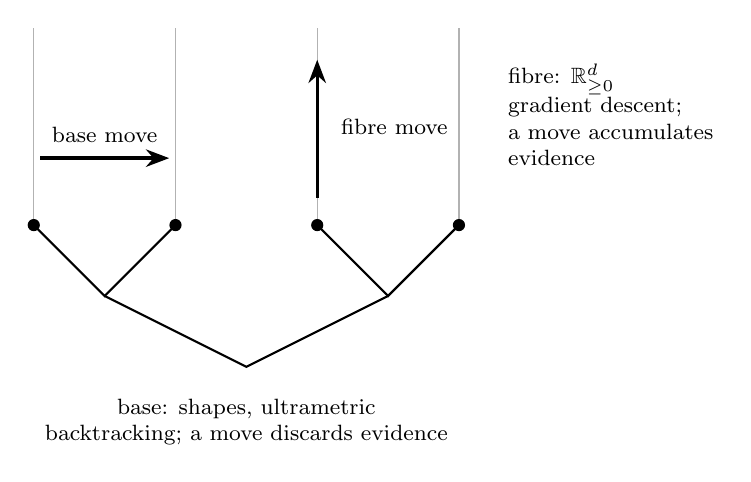
\begin{tikzpicture}[font=\small]
\foreach \x in {-2.7,-0.9,0.9,2.7} { \draw[gray!60] (\x,0) -- (\x,2.5); }
\foreach \x in {-2.7,-0.9,0.9,2.7} { \fill (\x,0) circle (2.2pt); }
\draw[thick] (-2.7,0) -- (-1.8,-0.9) -- (-0.9,0);
\draw[thick] (2.7,0) -- (1.8,-0.9) -- (0.9,0);
\draw[thick] (-1.8,-0.9) -- (0,-1.8) -- (1.8,-0.9);
\node[font=\footnotesize,align=center] at (0,-2.5)
  {base: shapes, ultrametric\\ backtracking; a move discards evidence};
\draw[very thick,-{Stealth}] (0.9,0.35) -- (0.9,2.1);
\node[font=\footnotesize,anchor=west] at (1.08,1.25) {fibre move};
\draw[very thick,-{Stealth}] (-2.62,0.85) -- (-0.98,0.85);
\node[font=\footnotesize,anchor=south] at (-1.8,0.92) {base move};
\node[font=\footnotesize,anchor=west,align=left] at (3.2,1.4)
  {fibre: $\Rnn^{d}$\\ gradient descent;\\ a move accumulates\\ evidence};
\end{tikzpicture}
\caption{Confinement is a theorem about the base. A fibre move has base-distance
zero, so it cannot leave a ball --- and can go anywhere inside one.}
\label{fig:fibration}
\end{figure}

\begin{principle}[Two searches, one learner]\label{prin:twosearch}
The base admits only backtracking search, priced by how far one had to back up;
the fibre admits gradient search, priced by the assays that produced the
evidence. A base move discards confirmations obtained below the depth of the
locus; a fibre move accumulates them. A learner needs both, and the two are not
interchangeable.
\end{principle}

\begin{remark}[What grading does not do]\label{rem:notescape}
It does not escape confinement. A learner that only revises values never leaves
the point it started at, let alone the ball. The forager of \S\ref{sec:robust} is
the illustration: it learns not to open, which saves its life, and it never
acquires a better test. Symmetrically, a learner that only moves in the base can
acquire deeper theories but pays for each, and --- as the companion note measures
--- may be made worse by depth while holding its other commitments fixed. Both
pathologies are visible in numbers, and neither is visible without the other
coordinate.
\end{remark}

%==============================================================================
\section{The gradient exists}\label{sec:gradient}

We now make Proposition~\ref{prop:fibration} operational. Three things are
required: that the fibre be smooth, that there be an objective whose gradient is
wanted, and that the gradient be computable by the learner rather than by an
observer of it.

\subsection{Clauses are posynomials}

\begin{definition}[Parameters]\label{def:params}
The \emph{parameters} of a graded clause are the constant symbols of $\V$
occurring in it. A clause with parameters $\theta = (\theta_1,\dots,\theta_d)$
and a candidate $\sigma$ determine a value $w(\theta,\sigma) \in \Rnn$.
\end{definition}

\begin{proposition}[Modality-free clauses are posynomials]\label{prop:posy}
Let $\psi$ be modality-free and fixed-point-free. Then for each candidate
$\sigma$,
\[
w(\theta,\sigma) \;=\; \sum_{i=1}^{N} c_i(\sigma)\,\prod_{j=1}^{d}
\theta_j^{\,a_{ij}},
\qquad c_i(\sigma)\in\{0,1\},\; a_{ij}\in\Nat ,
\]
a posynomial in $\theta$: the crisp subformulae contribute the coefficients and
the graded structure contributes the monomials. Consequently $w$ is smooth on the
positive orthant, and $\log w$ is convex as a function of $\log\theta$.
\end{proposition}

\begin{proof}
Induct on $\psi$. A constant is a monomial; $\crisp{\beta}$ is the constant $1$ or
$0$ according to whether $\beta$ holds at $\sigma$, since the guard evaluator is
pure and does not see $\theta$; $\tensorv$ is multiplication, which multiplies
monomials; $\sumv$ is addition, which concatenates the sums. Smoothness is
immediate. For log-convexity, write $\theta_j = e^{u_j}$; each monomial becomes
$e^{\langle a_i, u\rangle}$, so $w$ is a positive combination of exponentials of
affine functions, and the logarithm of such a combination is convex.
\end{proof}

\begin{proposition}[Normalisation is not log-convex]\label{prop:signomial}
The probability that a candidate fires within its contention set,
$p = w_\sigma / \sum_{\tau} w_\tau$, has $\log p = \log w_\sigma -
\log \sum_\tau w_\tau$, a difference of convex functions of $u = \log\theta$. It
is in general neither convex nor concave.
\end{proposition}

\begin{finding}[Curvature, measured]\label{find:curvature}
Over $400$ random modality-free clauses in $3$ parameters, evaluated at random
points of the positive orthant, the Hessian of $\log w$ in log-coordinates had
least eigenvalue $-8.882\times10^{-8}$ --- zero to the accuracy of the
finite-difference scheme, consistent with Proposition~\ref{prop:posy}. The
Hessian of $\log p$ was indefinite in $366$ of the same $400$ trials, with most
negative eigenvalue $-2.603$. Computed by \texttt{fibre.py}, experiment E4.
\end{finding}

The reading is the honest one. The fibre is smooth, so a gradient exists
everywhere on it, and clause values considered alone are as well behaved as a
geometric program. What is \emph{not} available is a guarantee that following the
gradient reaches a global optimum, because the act of normalising --- of turning
weights into a choice --- destroys convexity. A learner in this framework is
therefore in the ordinary position of a gradient learner: local moves, no
certificate.

\subsection{The likelihood of a causal history}

\begin{definition}[Causal history]\label{def:history}
A \emph{causal history} $h$ of length $\ell$ is a sequence of firings
$(\Gamma_1,\sigma_1),\dots,(\Gamma_\ell,\sigma_\ell)$, where each $\Gamma_i$ is a
contention set enabled at step $i$ and $\sigma_i$ a maximal matching of it,
quotiented by the interleaving of independent firings.
\end{definition}

The quotient is not a hygiene measure. Without it, $m$ independent firings
contribute the $m!$ linearisations of a partial order, and the likelihood
overcounts by that factor; the companion papers measure the inflation directly
and it is exactly $2, 6, 24$ for $m=2,3,4$. With it, the likelihood is well
defined:
\begin{equation}\label{eq:lik}
\Pr\nolimits_\theta(h) \;=\; \prod_{i=1}^{\ell}
\frac{w(\theta,\sigma_i)}{\sum_{\tau \in \Gamma_i} w(\theta,\tau)} .
\end{equation}

\begin{theorem}[The score decomposes over firing sites]\label{thm:score}
With $\Pr_\theta(h)$ as in \eqref{eq:lik},
\[
\frac{\partial}{\partial \theta_j}\log \Pr\nolimits_\theta(h)
\;=\;
\sum_{i=1}^{\ell}
\left(
\frac{\partial_j w(\theta,\sigma_i)}{w(\theta,\sigma_i)}
\;-\;
\frac{\sum_{\tau\in\Gamma_i}\partial_j w(\theta,\tau)}
     {\sum_{\tau\in\Gamma_i} w(\theta,\tau)}
\right).
\]
Each summand depends only on data local to the firing: the candidates of that
contention set, their clause values, their parameter derivatives, and which
matching fired.
\end{theorem}

\begin{proof}
Take logarithms in \eqref{eq:lik} and differentiate term by term; each term is a
difference of two logarithmic derivatives. Locality is by inspection: no factor
mentions a step other than its own.
\end{proof}

\begin{finding}[The decomposition, measured]\label{find:score}
Over $300$ random histories of $6$ contention sets each in $3$ parameters, the
worst discrepancy between the sum of local scores and a central-difference
gradient of the total log-likelihood was $1.221\times10^{-9}$. \texttt{fibre.py},
experiment E5.
\end{finding}

\begin{corollary}[The gradient is a message, not a pass]\label{cor:local}
A learner can accumulate $\partial_j \log \Pr_\theta(h)$ by adding one number per
firing to a running total. No global traversal of the reduction graph is
required, and nothing must be stored that the site did not already compute in
order to resolve its own race.
\end{corollary}

\begin{remark}[What this is, in other vocabularies]\label{rem:reinforce}
Theorem~\ref{thm:score} is the likelihood-ratio or score-function estimator; the
running total of Corollary~\ref{cor:local} is an eligibility trace; and combining
either with a terminal payoff is policy-gradient reinforcement learning. The
point of deriving rather than importing them is that here the policy is not a
neural network chosen for differentiability. It is the \texttt{where} clause, and
its differentiability is a consequence of Proposition~\ref{prop:posy}, which is a
consequence of the semiring. The learner's policy and the program's semantics are
the same object, so there is no interface between them to get wrong.
\end{remark}

\begin{remark}[Where the objective comes from]\label{rem:objective}
Nothing so far says what should be maximised. The framework answers this without
a hyperparameter: the learner has a token stack, the stack is conserved, and
running out of it ends the computation. The objective is therefore metabolic.
Which functional of the stack, however, is a genuine choice, and
\S\ref{sec:robust} reports two --- expected terminal stack and expected log
terminal stack --- side by side, because they disagree.
\end{remark}

\subsection{The modal case}\label{ssec:modal}

A clause bearing $\langle K\rangle_\V$ under a fixed point is not a posynomial,
and Proposition~\ref{prop:posy} does not apply. This is the case a learner
actually wants, because it is the case in which the clause is a hypothesis about
the future rather than about the datum in hand. It can be handled exactly.

\begin{definition}[The transfer operator]\label{def:transfer}
Over a finite set of configurations $\{1,\dots,n\}$, the graded modality is the
matrix $T$ with $T_{pq}$ the weight of the transition from $p$ to $q$. The clause
$\psi = \mu X.\,(\crisp{\beta} \sumv \langle K\rangle_\V X)$ denotes the least
solution $v$ of
\[
v \;=\; b + Tv, \qquad b_p = \text{value of } \crisp{\beta} \text{ at } p,
\]
which exists and equals $\sum_{i\ge0} T^i b$ when the spectral radius satisfies
$\varrho(T) < 1$.
\end{definition}

\begin{theorem}[The adjoint gives the gradient]\label{thm:adjoint}
Suppose $b$ and $T$ depend smoothly on $\theta$ and $\varrho(T) < 1$. Then $v$
depends smoothly on $\theta$ and
\[
(\mathrm{Id} - T)\,\partial_j v \;=\; \partial_j b + (\partial_j T)\,v ,
\qquad\text{hence}\qquad
\partial_j v \;=\; \sum_{i \ge 0} T^i\bigl(\partial_j b + (\partial_j T) v\bigr).
\]
The series on the right is the Neumann series of the same operator that defines
$v$. It converges under exactly the hypothesis that makes $v$ exist.
\end{theorem}

\begin{proof}
Differentiate $v = b + Tv$ with respect to $\theta_j$ and collect: $\partial_j v
= \partial_j b + (\partial_j T)v + T \partial_j v$. Since $\varrho(T)<1$,
$\mathrm{Id}-T$ is invertible with inverse $\sum_i T^i$, which gives both the
solution and its convergence; smoothness is the implicit function theorem applied
to $F(\theta,v) = v - b(\theta) - T(\theta)v$, whose partial derivative in $v$ is
$\mathrm{Id}-T$, invertible by hypothesis.
\end{proof}

\begin{corollary}[One condition, not two]\label{cor:onecond}
A modal graded clause over $\Rnn$ is differentiable in its parameters exactly
where it is defined. There is no separate regularity hypothesis for learning.
\end{corollary}

\begin{finding}[The adjoint, measured]\label{find:adjoint}
Over $200$ random systems of dimension $5$ in $2$ parameters with spectral radius
ranging over $[0.133, 0.952]$, the worst discrepancy between the adjoint solution
and a central-difference derivative of the fixed point was
$2.933\times10^{-8}$. Truncating the Neumann series at $60$ terms gives, at
spectral radius $0.50$, $0.90$, $0.99$, $1.00$ and $1.05$, the values
$2.000000$, $9.982030$, $45.284336$, $60.000000$ and $353.583718$ against exact
values $2.000000$, $10.000000$, $100.000000$ and divergence in the last two: the
approach to the boundary degrades value and gradient together.
\texttt{fibre.py}, experiment E6.
\end{finding}

\begin{remark}[Backpropagation, and what it is here]\label{rem:backprop}
Theorem~\ref{thm:adjoint} is reverse-mode differentiation through a fixed point,
and the practical recipe it licenses --- iterate the adjoint to the same
tolerance one iterated the value --- is the recipe used for implicit layers in
machine learning. What is worth noting is the direction of the derivation. There,
one designs a differentiable architecture and then studies its fixed points.
Here, the fixed point is what the logic already meant by a formula holding
henceforth, and its differentiability is a theorem about the semiring. The
learner does not have a differentiable model of its environment. It has a
hypothesis, and the hypothesis happens to be differentiable in its parameters.
\end{remark}

%==============================================================================
\section{Which gradient? The metric on the fibre}\label{sec:natgrad}

\subsection{The naive step is wrong, and wrong in a diagnosable way}

Fix the simplest interesting fibre. A learner holds one hypothesis of the shape
``a candidate satisfying the cheap structural test $\chi$ is worth acting on'',
and the clause value on such a candidate is a single parameter $\str \in (0,1)$.
Each time the learner acts it observes whether the candidate was in fact worth
acting on, an outcome $x \in \{0,1\}$. The obvious objective is the Bernoulli
log-likelihood
\[
\ell(\str; x) \;=\; x\log \str + (1-x)\log(1-\str),
\qquad
\Score(\str;x) \;\coloneqq\; \frac{\partial \ell}{\partial \str}
= \frac{x - \str}{\str(1-\str)} .
\]

Gradient ascent on $\ell$ is $\str \mapsto \str + \eta\,\Score(\str;x)$, and it is
a bad move for two reasons that are really one reason. It is unbounded near the
ends of the interval, so a confident learner meeting a surprise takes an enormous
step. And it is insensitive to how much evidence the current value rests on: a
learner that has seen one instance and a learner that has seen a thousand take
the same step on the next observation. Both faults are the absence of a metric.
The parameter $\str$ is a coordinate on a statistical manifold, and the Euclidean
geometry of the coordinate is not the geometry of the manifold.

\begin{definition}[The natural gradient]\label{def:natgrad}
The natural-gradient step with respect to a Riemannian metric $\Fish$ on the
parameter is $\str \mapsto \str + \eta\,\Fish^{-1}\Score$. Taking $\Fish$ to be
the Fisher information of the model is the canonical choice, and for $n$
independent Bernoulli observations it is
\[
\Fish(\str; n) \;=\; \frac{n}{\str(1-\str)} .
\]
\end{definition}

The Fisher information for a Bernoulli parameter is a count divided by a variance.
The variance cancels against the score. What is left is a count.

\subsection{The headline}

\begin{definition}[PLN simple truth values and revision]\label{def:pln}
A simple truth value is a pair $(\str, \ev)$ with $\str \in [0,1]$ a strength and
$\ev \ge 0$ an evidence count; the associated confidence is
$\conf = \ev/(\ev+k)$ for a personality parameter $k > 0$. Revision by a fresh
observation of strength $x$ and count $m$ is
\[
\mathrm{rev}\bigl((\str,\ev),(x,m)\bigr)
\;=\; \Bigl(\frac{\ev\str + m x}{\ev + m},\; \ev + m\Bigr).
\]
\end{definition}

\begin{theorem}[Revision is a natural-gradient step]\label{thm:natgrad}
For every $\str \in (0,1)$, every $\ev > 0$ and every $x$, the strength component
of $\mathrm{rev}((\str,\ev),(x,1))$ equals the natural-gradient ascent step on
the Bernoulli log-likelihood with unit step size and Fisher information evaluated
at the posterior count:
\[
\frac{\ev\str + x}{\ev+1}
\;=\;
\str + \Fish(\str;\ev+1)^{-1}\,\Score(\str;x).
\]
\end{theorem}

\begin{proof}
$\Fish(\str;\ev+1)^{-1}\Score(\str;x) = \dfrac{\str(1-\str)}{\ev+1}\cdot
\dfrac{x-\str}{\str(1-\str)} = \dfrac{x-\str}{\ev+1}$, and
$\str + \dfrac{x-\str}{\ev+1} = \dfrac{\ev\str + x}{\ev+1}$.
\end{proof}

\begin{finding}[The identity, measured, with its negative control]
\label{find:natgrad}
Over $20{,}000$ instances with $\str$ uniform on $[0.02,0.98]$, $\ev$ uniform on
$\{1,\dots,500\}$ and $x$ uniform on $\{0,1\}$, the worst absolute discrepancy
between revision and the natural-gradient step was $1.110\times10^{-16}$ with the
Fisher information taken at $\ev+1$, and $4.612\times10^{-1}$ with it taken at
$\ev$. The identification is therefore sharp: it is not merely that revision is
gradient-like, but that it is this step and not the neighbouring one.
\texttt{fibre.py}, experiment E1.
\end{finding}

\begin{corollary}[The step is implicit, hence stable]\label{cor:implicit}
Because the metric is evaluated after the increment, the update is the implicit
(backward-Euler, or proximal) discretisation of the natural gradient flow. It is
a convex combination of $\str$ and $x$ with weights $\ev/(\ev+1)$ and
$1/(\ev+1)$, so for $\ev > 0$ and $\str\in(0,1)$ the result lies strictly inside
the unit interval for every observation and every prior state. The explicit
discretisation does not have this property.
\end{corollary}

\begin{finding}[Stability, measured]\label{find:stable}
Over $200{,}000$ random steps with $\str$ uniform on $(0,1)$ and
$\ev \in \{1,\dots,50\}$:

\medskip
\begin{center}
\small
\begin{tabular}{lrrr}
\toprule
discretisation & escapes $[0,1]$ & absorbed & worst excursion \\
\midrule
implicit natural gradient (= revision) & $0$ & $0$ & $0.000$ \\
explicit natural gradient, step $1$ & $0$ & $3{,}882$ & $0.000$ \\
explicit natural gradient, step $1.5$ & $3{,}882$ & $0$ & $0.500$ \\
ascent on the raw score, step $1/(\ev+1)$ & $33{,}275$ & $0$ & $492.9$ \\
\bottomrule
\end{tabular}
\end{center}
\medskip

\noindent``Absorbed'' means the step landed exactly on $0$ or $1$, where the
score is undefined and no further observation can move the value.
\texttt{fibre.py}, experiment E2.
\end{finding}

The middle row deserves a comment, because it is the bootstrap trap of
\S\ref{sec:bootstrap} arriving by a different road. The explicit step with unit
size is $\str + (x-\str)/\ev$, which at $\ev = 1$ is exactly $x$: the learner's
first observation pins it to an endpoint, and an endpoint is absorbing. The
implicit step never reaches an endpoint because it always retains weight
$\ev/(\ev+1) > 0$ on where it was. Stability and the avoidance of dead
hypotheses are the same property.

\subsection{What has been derived}

\begin{principle}[Confidence is the metric, not a second value]
\label{prin:metric}
The resolution semantics of \S\ref{sec:algebra} needs a single number per
candidate, and it gets one: the clause is valued at the power $\str\conf$. The
learning dynamics needs, in addition, the geometry in which that number is to be
moved, and that geometry is a scalar field on the fibre --- the Fisher
information, which is the evidence count in disguise. So a PLN truth value is not
a two-dimensional value. It is a one-dimensional value together with the metric
at that point. Grading resolves; the metric learns.
\end{principle}

This settles, in the direction of the second option, a question the earlier note
left as a concession. There the observation was that PLN's revision is not a
semiring addition --- it is not idempotent, has no unit and does not distribute
--- and the recommendation was that $\Rnn$ supply the algebra while PLN supplied
values. That looked like a compromise. It is not: revision was never a candidate
for the algebra, because it is not an operation on values at all. It is a step in
a search over values, and steps in a search do not have to be semiring
operations. The apparent defect was a category error, and correcting it removes
the last piece of arbitrariness from the design.

\begin{remark}[Two coordinates, one of which is not observable at resolution]
\label{rem:cancel}
The earlier note also observed that confidence can be invisible: if the branch
competing with $\str\conf$ is the complement of the same belief, weighted
$(1-\str)\conf$, then normalisation gives
$\str\conf/(\str\conf + (1-\str)\conf) = \str$ and $\conf$ cancels exactly.
Principle~\ref{prin:metric} explains this rather than merely recording it. The
metric is not a value, so it does not appear in a ratio of values. It appears in
the \emph{step}, and a learner in that configuration still updates differently
according to $\conf$ even though it acts identically. Confidence becomes visible
in behaviour only when there is an outside option --- something to do other than
choose between two readings of one hypothesis --- because only then is the
absolute magnitude of $\str\conf$, rather than its ratio to itself, at stake.
\end{remark}

%==============================================================================
\section{The personality parameter is a step-size schedule}\label{sec:k}

\begin{definition}[The schedule]\label{def:schedule}
Along a sequence of observations the implicit step of
Corollary~\ref{cor:implicit} has size
$\eta_\ev = 1/(\ev+1)$, and if the learner begins with $k$ units of prior
evidence the schedule seen from the start is $\eta_j = 1/(j+k)$.
\end{definition}

\begin{proposition}[Robbins--Monro, for every $k$]\label{prop:rm}
For every $k>0$, $\sum_{j\ge1}\eta_j = \infty$ and
$\sum_{j\ge1}\eta_j^2 < \infty$.
\end{proposition}

\begin{proof}
$\sum 1/(j+k)$ diverges by comparison with the harmonic series and
$\sum 1/(j+k)^2$ converges by comparison with $\sum 1/j^2$; neither comparison
depends on $k$.
\end{proof}

\begin{finding}[The schedule, measured]\label{find:rm}
Truncating at $N = 200{,}000$:

\medskip
\begin{center}
\begin{tabular}{rrr}
\toprule
$k$ & $\sum_{j<N}\eta_j$ & $\sum_{j<N}\eta_j^2$ \\
\midrule
$1$ & $11.7833$ & $0.644929$ \\
$4$ & $10.7000$ & $0.221318$ \\
$9$ & $9.9544$ & $0.105161$ \\
$64$ & $8.0397$ & $0.015499$ \\
$512$ & $5.9693$ & $0.001946$ \\
\bottomrule
\end{tabular}
\end{center}
\medskip

\noindent The first column grows like $\log N$ for every $k$; the second is
bounded. \texttt{fibre.py}, experiment E3.
\end{finding}

\begin{corollary}[$k$ is a transient parameter]\label{cor:transient}
Under the standard stochastic-approximation hypotheses the schedule converges for
every $k$, so $k$ does not determine whether the learner arrives, only how it
travels. An immortal learner is therefore indifferent to $k$.
\end{corollary}

\begin{principle}[Only mortality can price the learning rate]\label{prin:pricek}
Since every $k$ converges, no purely statistical criterion selects one. A learner
with a finite stack that can be exhausted during the transient is a criterion:
it is harmed by excursions it does not survive, and rewarded for opportunities it
takes early enough to profit from. So the choice of $k$ --- which in the
probabilistic-logic literature is set by taste, and named for taste --- acquires
a selection criterion exactly when the learner is embedded in an ecology that can
kill it.
\end{principle}

This is the point at which the traffic runs both ways. The framework gains a
principled derivation of PLN; PLN gains a criterion for the one parameter it
could not otherwise justify. \S\ref{sec:robust} measures it.

%==============================================================================
\section{The bootstrap trap is a vanishing gradient}\label{sec:bootstrap}

\begin{proposition}[Zero is absorbing]\label{prop:zero}
Suppose a learner's only way of acquiring evidence about $\psi$ is to fire the
receipt guarded by $\psi$, and suppose $\psi$ evaluates to $0$ on every
candidate. Then by Definition~\ref{def:comm} the receipt offers no transition, so
it never fires, so no evidence arrives, so $\psi$ is never revised. The state is
a fixed point of the learning dynamics, and it is not a local optimum of
anything.
\end{proposition}

\begin{corollary}[The trap, concretely]\label{cor:trap}
With $\conf = \ev/(\ev+k)$ and $\ev_0 = 0$ we get $\conf = 0$, hence
$\pow = \str\conf = 0$, hence a continuously enabled receipt that never fires.
A learner initialised with no prior evidence at all does not die; it does
nothing.
\end{corollary}

\begin{finding}[Stasis, measured]\label{find:trap}
In the baseline ecology of \S\ref{sec:robust}, the arm initialised at $\ev_0=0$
opens nothing, ends with $\str$ unchanged at $0.5000$, and terminates with a mean
stack of $520.0$, which is exactly the value of grazing and never acting. The
same learner with one unit of prior evidence reaches a mean terminal stack of
$716.7$. Survival in the first case is $1.0000$: the trap is not lethal, which is
what makes it hard to see.
\end{finding}

In gradient vocabulary this is a dead unit, and the diagnosis is the standard
one: the score is undefined where the branch probability is zero, so the learner
sits at a point at which its own gradient does not exist. What is unusual is that
the framework supplies both standard remedies \emph{inside the clause language},
so that neither is a training-loop artefact bolted onto the semantics.

\begin{definition}[Two repairs, both written as formulae]\label{def:repairs}
\emph{Initialisation}: require $\ev_0 \ge 1$, which is prior evidence and is
stated as part of the hypothesis.
\emph{Exploration}: replace $\psi$ by $\psi \sumv \varepsilon$ for a constant
$\varepsilon > 0$, a graded disjunction guaranteeing a floor on the weight.
\end{definition}

\begin{principle}[Exploration is a disjunct]\label{prin:explore}
The exploration bonus of a reinforcement learner is, in this setting, the
statement that the learner will act if its hypothesis says so \emph{or} for no
reason. It is a connective of the hypothesis language, not a parameter of a
training procedure, and it is priced like any other disjunct: the $\varepsilon$
branch fires at a rate the ecology charges for.
\end{principle}

\begin{remark}[The other end of the same axis]\label{rem:otherend}
The trap is what happens as the weight tends to zero. \S\ref{sec:robust} exhibits
the opposite end, where a very large $k$ suppresses the weight almost as
effectively and the learner's behaviour becomes nearly indistinguishable from the
trapped one. Between them lies whatever interior optimum the ecology allows, and
part of the value of measuring it is finding out how narrow the interval is.
\end{remark}

%==============================================================================
\section{The price of the transient, measured across an ecology}
\label{sec:robust}

\subsection{Why the sweep is over distributions and not over payoffs}

An earlier version of this material fixed a payoff table --- a probability that a
specimen is rich, a pair of likelihoods for the cheap test, two stack sizes ---
and varied one number at a time. A referee's objection to that was correct and
worth restating: a synthetic decision problem in which a tunable parameter
develops an interior optimum shows that \emph{this} decision problem has one. It
establishes nothing general.

The repair is not to add more payoff tables but to change what is being varied.
The companion programme does not describe environments by payoffs. It describes
them by three distributions, and those three are what specify an ecology:

\begin{description}[leftmargin=1.6em,itemsep=2pt]
\item[(T) the distribution over trophic types.] Among the computations that can
be opened at all, some are \emph{autotrophs} --- they draw only on free reservoirs
and have accumulated little; some are \emph{heterotrophs} --- they eat other
computations, and have therefore accumulated much; and some are composites, which
do both. The trophic type is an access profile, not a species: it is a fact about
what a computation's cut permits.
\item[(I) the distribution over inedibles.] Computations that cannot be opened at
a profit. They are not decoys planted by an experimenter; they are the ordinary
residue of an ecology in which most things are not food.
\item[(R) the distribution over token reservoirs housed in no trophic type.] Free
stacks --- the wall. Non-exclusive, rate-limited, and the learner's outside
option.
\end{description}

Varying these is varying the ecology rather than the puzzle, and the question
``does the interior optimum survive?'' becomes a question about which ecologies
support learners of which temperament.

\subsection{The setting}

A forager senses at a price $\kappa_{\mathrm{sense}} = 4$, meets a free reservoir
with probability $R$ yielding $5$, and otherwise meets a computation drawn from
the composition $(T, I)$. It observes the cheap structural predicate $\chi$, the
presence of harvesting apparatus, whose likelihood varies by type:
\[
\Pr(\chi \mid \text{hetero}) = 0.85,\quad
\Pr(\chi \mid \text{comp}) = 0.75,\quad
\Pr(\chi \mid \text{auto}) = 0.45,\quad
\Pr(\chi \mid \text{inedible}) = 0.30 .
\]
Holdings are $\sigma = 130, 70, 30, 0$ for the four kinds, and breaking in costs
$\kappa_{\mathrm{break}} = 60$; so heterotrophs and composites are profitable and
autotrophs and inedibles are not. The learner's hypothesis is
$\mathrm{Inheritance}(\chi, \mathrm{Profitable})$, held as $(\str,\ev)$ and
placed in the \texttt{where} clause of the break-in receipt at the power
$\str\conf$, racing the graze branch at fixed weight $g = 0.5$. Endowment $120$,
horizon $400$. Two openings of headroom: an early mistake is close to fatal,
which is what puts the transient of \S\ref{sec:k} on the critical path.

\begin{center}
\begin{tabular}{lrrrr}
\multicolumn{5}{c}{\emph{Baseline ecology}: $T = 0.40$, $I = 0.40$, $R = 0.25$,}\\
\multicolumn{5}{c}{$\Pr(\mathrm{Profitable}\mid\chi) = 0.6278$,
$E[\text{net}\mid\text{open}] = +11.11$}\\[4pt]
\toprule
arm & survival & wealth & log-fitness & final $\str$ \\
\midrule
naive ($\ev_0 = 0$) & $1.0000$ & $520.0$ & $6.2558$ & $0.5000$ \\
crisp & $0.4384$ & $626.2$ & $3.1374$ & $0.4801$ \\
individual ($\ev$ capped) & $0.6851$ & $604.5$ & $4.5755$ & $0.5661$ \\
graded, $k=4$ & $0.6128$ & $716.7$ & $4.2652$ & $0.5313$ \\
\bottomrule
\end{tabular}
\end{center}

\smallskip
\noindent The crisp arm is the note as it stood before grading: a Boolean guard
that fires whenever $\chi$ holds. It has the highest wealth conditional on
surviving and much the worst survival, which is the earlier finding reproduced in
a different world --- a Boolean guard has no coordinate in which to record
disappointment, so it cannot learn to stop. The naive arm is the bootstrap trap.

\subsection{Two objectives, side by side}

\begin{center}
\begin{tabular}{rrrr}
\toprule
$k$ & survival & wealth & log-fitness \\
\midrule
$0.5$ & $0.5122$ & $646.0$ & $3.6037$ \\
$1$ & $0.5283$ & $658.4$ & $3.7116$ \\
$2$ & $0.5512$ & $676.0$ & $3.8625$ \\
$4$ & $0.6082$ & $711.0$ & $4.2345$ \\
$9$ & $0.7133$ & $\mathbf{744.6}$ & $4.8794$ \\
$16$ & $0.8260$ & $738.5$ & $5.5164$ \\
$32$ & $0.9537$ & $670.6$ & $6.1568$ \\
$64$ & $0.9952$ & $575.0$ & $\mathbf{6.2869}$ \\
$128$ & $0.9998$ & $536.4$ & $6.2717$ \\
$256$ & $1.0000$ & $525.3$ & $6.2612$ \\
$512$ & $1.0000$ & $522.2$ & $6.2580$ \\
\bottomrule
\end{tabular}
\end{center}

\begin{finding}[The two criteria select different learners]\label{find:twoobj}
In the baseline ecology the optimum under expected terminal stack is $k^* = 9$,
with survival $0.7133$; the optimum under expected log terminal stack is
$k^* = 64$, with survival $0.9952$. The two differ by a factor of seven, and the
learner preferred by one criterion is killed three times as often as the learner
preferred by the other. \texttt{ecology.py}.
\end{finding}

Neither criterion is obviously wrong, and it is worth being explicit about what
each is for. Expected terminal stack is the right question if the learner is one
draw from a population whose aggregate holdings matter and whose individual
deaths do not. Expected log terminal stack is the right question if the learner
is a single lineage in a multiplicative process with an absorbing barrier, which
is what a mortal computation with a conserved stack actually is. The framework
does not adjudicate; it makes the disagreement visible and prices both sides.

\begin{finding}[The criteria disagree about whether learning pays at all]
\label{find:worthit}
Under expected wealth the best graded forager reaches $744.6$ against the
do-nothing forager's $520.0$, a gain of $43\%$. Under log-fitness the best graded
forager reaches $6.2869$ against the do-nothing forager's $6.2558$, a margin of
$0.031$ --- and every $k \ge 128$ scores below $6.2717$, converging on the
do-nothing value from above. In this ecology the log criterion can barely
distinguish a learner from a learner that never acts.
\end{finding}

That finding is the honest centre of this section, and it sharpens
Remark~\ref{rem:otherend}. The trap at $\ev_0 = 0$ and the trap at $k \to \infty$
are the same trap approached from two directions, and under a criterion that
rewards survival above all, both look excellent. A framework that reports only
log-fitness would conclude that the best policy is to do nothing, and it would be
right about survival and wrong about everything else.

\subsection{The three sweeps}

Each sweep varies one distribution and holds the others at the baseline.
``$k^*(w)$'' is the optimum under expected wealth, ``$k^*(\ell)$'' under
log-fitness, each with the survival it achieves; $3000$ lives per cell, eleven
values of $k$ per cell.

\begin{center}
\begin{tabular}{rrrrrrr}
\multicolumn{7}{c}{\emph{(T) the distribution over trophic types}: heterotroph
share among edibles}\\[3pt]
\toprule
$T$ & $\Pr(\mathrm{Prof}\mid\chi)$ & $k^*(w)$ & survival & $k^*(\ell)$ & survival
& $E[\text{net}]$ \\
\midrule
$0.00$ & $0.4687$ & $512$ & $1.0000$ & $512$ & $1.0000$ & $-18.75$ \\
$0.20$ & $0.5529$ & $512$ & $1.0000$ & $512$ & $1.0000$ & $-2.94$ \\
$0.40$ & $0.6278$ & $9$ & $0.7123$ & $64$ & $0.9943$ & $+11.11$ \\
$0.60$ & $0.6947$ & $4$ & $0.8223$ & $16$ & $0.9313$ & $+23.68$ \\
$0.80$ & $0.7550$ & $1$ & $0.8507$ & $16$ & $0.9620$ & $+35.00$ \\
$1.00$ & $0.8095$ & $2$ & $0.9117$ & $9$ & $0.9633$ & $+45.24$ \\
\bottomrule
\end{tabular}
\end{center}

\begin{center}
\begin{tabular}{rrrrrrr}
\multicolumn{7}{c}{\emph{(I) the distribution over inedibles}}\\[3pt]
\toprule
$I$ & $\Pr(\mathrm{Prof}\mid\chi)$ & $k^*(w)$ & survival & $k^*(\ell)$ & survival
& $E[\text{net}]$ \\
\midrule
$0.00$ & $0.8071$ & $0.5$ & $0.9683$ & $4$ & $0.9860$ & $+31.43$ \\
$0.20$ & $0.7290$ & $1$ & $0.8297$ & $16$ & $0.9610$ & $+22.58$ \\
$0.40$ & $0.6278$ & $9$ & $0.7123$ & $64$ & $0.9943$ & $+11.11$ \\
$0.60$ & $0.4913$ & $512$ & $1.0000$ & $512$ & $1.0000$ & $-4.35$ \\
$0.80$ & $0.2974$ & $512$ & $1.0000$ & $512$ & $1.0000$ & $-26.32$ \\
\bottomrule
\end{tabular}
\end{center}

\begin{center}
\begin{tabular}{rrrrrrr}
\multicolumn{7}{c}{\emph{(R) the distribution over free reservoirs}}\\[3pt]
\toprule
$R$ & $\Pr(\mathrm{Prof}\mid\chi)$ & $k^*(w)$ & survival & $k^*(\ell)$ & survival
& $E[\text{net}]$ \\
\midrule
$0.00$ & $0.6278$ & $16$ & $0.7267$ & $128$ & $0.9983$ & $+11.11$ \\
$0.15$ & $0.6278$ & $9$ & $0.6807$ & $128$ & $0.9993$ & $+11.11$ \\
$0.30$ & $0.6278$ & $9$ & $0.7463$ & $64$ & $0.9977$ & $+11.11$ \\
$0.45$ & $0.6278$ & $9$ & $0.8300$ & $32$ & $0.9870$ & $+11.11$ \\
$0.60$ & $0.6278$ & $9$ & $0.9147$ & $32$ & $0.9940$ & $+11.11$ \\
\bottomrule
\end{tabular}
\end{center}

\subsection{Interaction between two of the distributions}

The sweeps above vary one distribution at a time. Because (T) and (I) both enter
the conditional $\Pr(\mathrm{Prof}\mid\chi)$, they might be expected to interact,
and a coarser grid over the pair confirms that they do --- and that the
interaction is legible. Cells use $1200$ lives, so the optima are noisier than in
the sweeps; the baseline cell reports $k^*(w) = 16$ here against $9$ at the
higher count.

\begin{center}
\begin{tabular}{rrrrrr}
\toprule
$T$ & $I$ & $\Pr(\mathrm{Prof}\mid\chi)$ & $E[\text{net}]$ & $k^*(\ell)$ & $k^*(w)$ \\
\midrule
$0.15$ & $0.15$ & $0.646$ & $+4.6$ & $512$ & $512$ \\
$0.15$ & $0.40$ & $0.533$ & $-6.7$ & $512$ & $512$ \\
$0.15$ & $0.70$ & $0.334$ & $-26.6$ & $512$ & $512$ \\
$0.40$ & $0.15$ & $0.750$ & $+25.0$ & $16$ & $1$ \\
$0.40$ & $0.40$ & $0.628$ & $+11.1$ & $64$ & $16$ \\
$0.40$ & $0.70$ & $0.404$ & $-14.3$ & $512$ & $512$ \\
$0.75$ & $0.15$ & $0.870$ & $+48.4$ & $9$ & $1$ \\
$0.75$ & $0.40$ & $0.741$ & $+32.3$ & $16$ & $2$ \\
$0.75$ & $0.70$ & $0.492$ & $+1.3$ & $512$ & $512$ \\
\bottomrule
\end{tabular}
\end{center}

\subsection{What the surface says}

\begin{finding}[The interior optimum requires a margin, not merely a profit]
\label{find:interior}
Across all $25$ cells reported above, the two optima agree about which side of the
grid they fall on. Every cell with $E[\text{net}\mid\text{open}] \ge +11.1$ has an
interior optimum under both objectives; every cell with
$E[\text{net}\mid\text{open}] \le +4.6$ has a boundary optimum under both. Sixteen
cells are interior and nine are at the boundary, and no cell in the measured
range lies between $+4.6$ and $+11.1$.
\end{finding}

Two of the boundary cells --- $(T,I) = (0.15,0.15)$ at $+4.6$ and
$(0.75,0.70)$ at $+1.3$ --- have \emph{positive} expected net yield from opening
and still send the personality parameter to maximal scepticism. That is the
finding worth having, and it is stronger than the one anticipated. Positive
expectation is not sufficient to make acting worthwhile for a learner that can
die. With two openings of headroom, a thin positive mean is dominated by the
variance around it, and the correct policy is abstention. The threshold is
therefore strictly positive, and where it sits is a joint property of the
ecology's payoffs and the learner's endowment --- which is the Kelly criterion
arriving from the ecological side rather than the financial one.

This is also the correct and modest version of the earlier claim about an
interior optimum. There is no general interior optimum for the personality
parameter. There is one exactly when the ecology makes acting worth doing by a
margin, and where it does not, maximal scepticism is not a failure of nerve but
the right answer --- the boundary optimum is the framework saying so. What
survives robustness is not the number but the criterion.

\begin{finding}[Scepticism and free energy are substitutes]\label{find:substitute}
Along the (R) sweep the hypothesis being learned does not change: the truth
$\Pr(\mathrm{Prof}\mid\chi)$ is $0.6278$ in every cell, because free reservoirs
are not computations and do not enter the conditional. Yet $k^*(\ell)$ falls from
$128$ to $32$ as reservoirs become abundant, and survival at the wealth optimum
rises from $0.6807$ to $0.9147$.
\end{finding}

\begin{principle}[The transient is what an outside option pays for]
\label{prin:outside}
A rich outside option does not make the learner's hypothesis truer or its test
sharper. It makes the transient survivable, by supplying income the learner does
not have to gamble for. Scepticism is the other way of surviving a transient, so
the two trade off, and an ecology with abundant free energy can afford credulous
learners. This is a statement about environments, not about learners, and it is
statable only because the framework prices perception, action and survival in one
currency.
\end{principle}

\begin{remark}[What is not claimed]\label{rem:notclaimed}
These are measurements on a constructed ecology with four kinds of computation, a
single binary structural predicate, and a fixed price schedule. What has been
established is the shape of the dependence --- which way $k^*$ moves as each
distribution moves, and where the interior optimum stops existing --- not a
quantitative law. The numbers are reproducible from \texttt{ecology.py} and should
be read as the behaviour of that model.
\end{remark}

%==============================================================================
\section{Where the gradient cannot go}\label{sec:base}

Everything in \S\S\ref{sec:gradient}--\ref{sec:robust} happens in one fibre. The
learner tunes $\theta$, and $\theta$ is the value of a hypothesis whose
\emph{shape} it never questions. It is worth being explicit about how severe that
restriction is, because the machinery is seductive and the restriction is not
visible from inside it.

\begin{proposition}[The fibre gradient never changes the theory]\label{prop:nobase}
Let $(\psi,\theta) \mapsto (\psi,\theta')$ be any sequence of fibre moves. Then
the base component is constant, so by Proposition~\ref{prop:tree} the ultrametric
distance travelled is $0$, and by Proposition~\ref{prop:confinement} the learner
remains in every ball it started in --- including the ball of radius $0$.
\end{proposition}

A learner equipped only with gradient descent is confined absolutely. It is not
slow to escape a bad theory; it cannot form the question. The forager of
\S\ref{sec:robust} is the illustration and it is a sharp one: it learns
beautifully not to open inedibles, and in four hundred steps it never once
considers that a second structural predicate might separate heterotrophs from
autotrophs, which is the hypothesis that would actually pay.

\begin{principle}[What the fibre buys, exactly]\label{prin:fibrebuy}
Before grading, the only way to change behaviour was to change the formula: a
discrete jump, priced by backtracking depth, invalidating every confirmation
obtained below that depth. After grading, behaviour can be changed continuously
while the formula and the evidence are held fixed. Grading does not enlarge the
set of reachable theories by one element. It makes the interior of a ball
navigable, and \S\ref{sec:robust} measures what that is worth: in the harsh cells
it is the difference between abstention and extinction.
\end{principle}

\subsection{What escapes}

Three operators move in the base, and all three are structural rather than
epistemic. They are treated in the companion notes and are recalled here only to
place them relative to the gradient.

\emph{Recombination.} Reproduction by crossover on quoted code is a base move of
arbitrary size. Because a germ is a quotation --- inert, transmissible,
inspectable --- crossover can exchange whole subformulae, which is precisely the
move an incremental revision walk cannot make. The transport claim of the
scientist note, that a revision move and a crossover are one move carried along
the characteristic-formula map and distinguished only by accessible distance, is
what makes this a statement about the same space rather than an analogy.

\emph{Composition.} Two learners in parallel constitute a learner whose namespace
is the union, and disjointness of namespaces is exactly probabilistic
independence of their distributions. Composition therefore reaches shapes neither
component could reach, at the price of the interaction term.

\emph{Death.} A population in which lineages end is a search that can abandon a
ball, which no individual can do.

\begin{principle}[The division of labour is forced by the geometry]
\label{prin:division}
Continuous parameter learning and discrete structure search are not two design
choices made by an engineer who could have made others. They are what the two
components of a fibration respectively admit: an ordered continuum has nothing
but gradients, and an ultrametric has none. A framework in which hypotheses are
formulae and confidences are numbers must have gradient descent on the numbers
and evolutionary or backtracking search on the formulae, and it must have both
because neither reaches what the other reaches.
\end{principle}

That this reproduces the familiar arrangement --- stochastic gradient descent
over parameters, discrete search over architectures --- is worth saying plainly,
because the point is the direction of the derivation. The arrangement is not
imported here as good practice. It is a consequence of the geometry of a
hypothesis space whose points are formulae, and the framework predicts it rather
than assuming it.

%==============================================================================
\section{Testimony, and the conservation of evidence}\label{sec:testimony}

\subsection{Two conservation laws, one of which is false}

Tokens are conserved. The game rules of the companion programme are explicit
about it: a stack may be moved, split, or spent, and never minted, and the whole
economics of the mortal scientist rests on that.

Evidence is not conserved. Nothing in the framework prevents a learner from
counting the same observation twice, and PLN revision --- which by
Theorem~\ref{thm:natgrad} is the fibre's gradient step --- presumes that the
evidence it is handed is independent of the evidence it already has. Two learners
who both heard from a third and then revise by each other's truth values have
double-counted, and the arithmetic cannot tell.

\begin{principle}[Belief inflation is minting]\label{prin:minting}
The metabolic namespace has a conservation law and the belief namespace does not.
So the epistemic analogue of counterfeiting exists, has no metabolic analogue,
and requires no defect in any participant: honest agents running the correct
update rule on correlated evidence inflate the count.
\end{principle}

\subsection{What inflation does, in gradient terms}

The natural reading of counterfeit confidence is recklessness --- an agent that
believes too strongly and acts too boldly. Theorem~\ref{thm:natgrad} says the
opposite, and the prediction is sharp enough to test.

\begin{proposition}[Inflation collapses the step size]\label{prop:freeze}
The evidence count is the Fisher information up to the variance factor, and the
step size is $\eta = 1/(\ev+1)$. Inflating $\ev$ by a factor $\lambda$ therefore
divides the learner's step size by approximately $\lambda$. A learner with
counterfeit confidence is not unstable. It is rigid.
\end{proposition}

\begin{corollary}[The damage is invisible in a stationary world]\label{cor:invisible}
If the truth being estimated does not move, a collapsed step size costs almost
nothing: the learner has already converged to approximately the right value and
is merely unable to move away from it. The cost of minted confidence appears only
when the environment changes, and it appears as an inability to re-adapt.
\end{corollary}

\subsection{The experiment}

Two learners share a belief namespace. Each forages a stretch of the horizon and
then, in some protocols, exchanges truth values with the other. Three protocols:

\begin{description}[leftmargin=1.6em,itemsep=2pt]
\item[isolated] no exchange;
\item[honest] one exchange at the midpoint, of evidence drawn from disjoint
streams, so counts add and the sum is warranted;
\item[plagiarism] exchange at every epoch, so that each learner's count is
re-transmitted and re-added on the following exchange, and the same observations
circulate.
\end{description}

The ecology is the baseline of \S\ref{sec:robust} with $k = 9$, run in two
regimes: one in which the trophic composition shifts at the midpoint from
$(T,I) = (0.40,0.40)$ to $(0.05,0.65)$, moving the truth from $0.6278$ to
$0.3409$, and a stationary control. ``Inflation'' is the ratio of the nominal
evidence count to the count actually warranted by distinct observations.

\begin{center}
\begin{tabular}{lrrrrrr}
\multicolumn{7}{c}{\emph{Shifting ecology}: truth $0.6278 \to 0.3409$ at the
midpoint}\\[3pt]
\toprule
protocol & inflation & $|\str-\text{truth}|$ & $|\str-\text{truth}|$ &
step & survival & wealth \\
 & $\ev/\ev_{\mathrm{indep}}$ & pre-shift & post-shift & $1/(\ev+1)$ & & \\
\midrule
isolated & $1.000$ & $0.1246$ & $\mathbf{0.1573}$ & $0.05295$ & $0.1590$ & $68.4$ \\
honest & $1.000$ & $\mathbf{0.0706}$ & $0.2052$ & $0.02183$ & $0.1307$ & $62.2$ \\
plagiarism & $\mathbf{140.98}$ & $0.0752$ & $0.2446$ & $0.00043$ & $0.1183$ & $61.7$ \\
\bottomrule
\end{tabular}
\end{center}

\begin{center}
\begin{tabular}{lrrrrrr}
\multicolumn{7}{c}{\emph{Stationary control}: truth $0.6278$ throughout}\\[3pt]
\toprule
protocol & inflation & $|\str-\text{truth}|$ & $|\str-\text{truth}|$ &
step & survival & wealth \\
 & $\ev/\ev_{\mathrm{indep}}$ & first half & second half & $1/(\ev+1)$ & & \\
\midrule
isolated & $1.000$ & $0.1197$ & $0.0982$ & $0.04213$ & $0.7350$ & $772.3$ \\
honest & $1.000$ & $\mathbf{0.0703}$ & $\mathbf{0.0583}$ & $0.01815$ & $0.7213$ & $766.2$ \\
plagiarism & $133.52$ & $0.0747$ & $0.0699$ & $0.00042$ & $0.6637$ & $754.6$ \\
\bottomrule
\end{tabular}
\end{center}

\subsection{Four findings}

\begin{finding}[Honest testimony is superadditive, and cheap]\label{find:honest}
One exchange of independent evidence reduces the error in $\str$ from $0.1246$ to
$0.0706$ in the shifting run and from $0.1197$ to $0.0703$ in the control ---
close to the factor $\sqrt{2}$ that doubling independent evidence predicts --- at
no metabolic cost to either party beyond the message. This is the inequality
behind the slogan that cooperation is epistemic and competition metabolic, with a
number attached.
\end{finding}

\begin{finding}[Plagiarism buys accuracy nothing and count everything]
\label{find:plagiarism}
The plagiarism protocol reaches pre-shift error $0.0752$, no better than the
single honest exchange's $0.0706$, while its nominal evidence count is inflated
by a factor of $140.98$. Confidence has been minted at a ratio of one hundred and
forty to one against the evidence backing it.
\end{finding}

\begin{finding}[The pathology is rigidity, and it is invisible until the world
moves]\label{find:rigid}
Step sizes at the end of the run are $0.05295$, $0.02183$ and $0.00043$ for the
three protocols. In the stationary control the ordering of post-period accuracy
follows accuracy, as one would hope: honest $0.0583$, plagiarism $0.0699$,
isolated $0.0982$. In the shifting run the ordering \emph{inverts} and follows
step size instead: isolated $0.1573$, honest $0.2052$, plagiarism $0.2446$. The
plagiarists are the least able to notice that the world has changed, exactly as
Proposition~\ref{prop:freeze} predicts, and the honest sharers are second-least
able.
\end{finding}

The second half of that finding is the uncomfortable one and should not be
softened. Under a regime shift, \emph{any} accumulation of evidence is a
liability, and honest testimony is a liability too --- smaller than counterfeit
testimony, larger than isolation. The Robbins--Monro schedule is designed for a
stationary target. A mortal learner in a changing ecology is not solving that
problem, and the framework makes the mismatch measurable rather than concealing
it. The obvious repair, discounting old evidence so that $\eta$ has a floor, is
not innocent either: it is a step size that does not satisfy
Proposition~\ref{prop:rm}, so it trades convergence for plasticity.

\begin{finding}[Accuracy and fitness come apart, with a sign]\label{find:apart}
In both regimes the metabolic ordering is the reverse of the epistemic one:
isolated learners hold the most wealth ($772.3$ in the control) and the most
accurate learners the least ($754.6$ for plagiarism, $766.2$ for honest exchange),
and survival follows wealth. In a marginal ecology --- one where
$E[\text{net}\mid\text{open}]$ is positive but thin --- converging quickly to the
true strength means acting on it, and acting on a thin edge is expensive. The
earlier programme's slogan that a learner is paid in yield and not in truth is
reproduced here independently, and with the additional detail that testimony
sharpens truth while slightly degrading yield.
\end{finding}

\begin{remark}[What the two-learner run does not settle]\label{rem:testimonyopen}
The protocols here are stipulated rather than chosen by the learners. Whether a
population in which testimony is available has an equilibrium, and whether
plagiarism invades it, requires the belief to be a strategy and the exchange to be
priced --- which is composition in the sense of the companion note, and is left
open. Nor is any defence attempted: an evidence-provenance discipline that made
double counting detectable would be the belief-namespace analogue of the
conservation law the metabolic namespace already has, and the framework says
clearly what it would have to do, but not how.
\end{remark}

%==============================================================================
\section{Implementation}\label{sec:impl}

Three pieces of what is described here already exist, one does not, and the
boundary is worth being precise about.

\paragraph{The clause.} The \texttt{where} clause is present in the reference
node as field \texttt{condition} of the receive form, evaluated in the matcher by
a separate pure-evaluation crate. Per-match evaluation is what the matcher
already does, since a guard must be checked against the bindings a candidate
supplies. Making the clause $\Rnn$-valued rather than Boolean is a change of
codomain in one function, and the classical interpreter can continue to read only
the support --- fires if non-zero --- so a graded program remains a legal
classical program.

\paragraph{The simulator.} The weighted-GSLT crate carries rules equipped with
weight maps keyed by spatial-behavioural formulae, computes propensities by
redex, and runs both a classical stochastic simulation and a quantum one. Its
weight maps are, by the normal-form theorem of Paper~III, graded clauses in
disjunctive form, so it is already an implementation of the special case. What it
does not have is a clause language: the keys are a hand-rolled formula enum and
the partition discipline it enforces is exactly the discipline a single-valued
clause makes unnecessary.

\paragraph{The gradient.} Corollary~\ref{cor:local} says what a runtime would
have to carry, and it is little. At each firing, the site already computed the
weight of every candidate in its contention set in order to resolve the race. To
accumulate the score it must additionally compute, for each parameter, the
derivative of each candidate weight --- available in closed form from
Proposition~\ref{prop:posy}, since a posynomial's derivative is a posynomial ---
and add one number per parameter to a running total. That total is an eligibility
trace, and in \rhoc{} the natural place for it is a message on a channel private
to the learner, which makes it harvestable like any other belief. Nothing
requires a backward pass over the reduction graph, and nothing requires the graph
to be retained.

\paragraph{The belief.} Because a truth value sits on a channel as data, revision
is an ordinary communication and Remark~\ref{rem:plastic} does the rest. The
consequence noticed in the earlier note stands and is sharpened by
\S\ref{sec:testimony}: a belief is a message, so testimony and the theft of a
hypothesis are the same operation as predation, differing only in which namespace
the name lives in.

\paragraph{What is not built.} None of the gradient machinery. The scripts
shipped with this note are simulations of the mathematics, not instrumentation of
a node: \texttt{fibre.py} verifies the identities and \texttt{ecology.py} runs the
foragers, and neither executes \rhoc{}.

%==============================================================================
\section{Related work}\label{sec:related}

\paragraph{Semiring-weighted computation.} Weighting the transitions of a system
by elements of a semiring, multiplying along paths and summing across them, is
long established --- weighted automata are the canonical instance, and
semiring-valued logics predate this line of work by decades. Nothing in the
algebra of \S\ref{sec:algebra} is new, and the earlier version of this material
was rightly criticised for not saying so.

\paragraph{Stochastic process calculi.} Rates attached to actions, with races
resolved by relative rate and holding times drawn from the total, are the design
of the stochastic pi calculus and its machine, and of the performance-evaluation
calculi. The differences here are two. The weight is attached to a
\emph{candidate match} rather than to a channel or an action, so it may depend on
the datum; and it is written as a formula of a logic generated by the term
language rather than as a numeral, which is what makes it something a learner can
hold as a hypothesis.

\paragraph{The novelty claim.} Stated narrowly, and following a reviewer's own
sharpening: placing a semiring-valued expression exactly at \rhoc{}-calculus
candidate-match resolution. What this paper adds to that claim is the reading of
the resulting parameter as the fibre of a fibration over the hypothesis lattice,
and the identification of the metric on that fibre.

\paragraph{Probabilistic logic networks.} PLN supplies the truth-value structure
of \S\ref{sec:natgrad}: a strength, an evidence count, a confidence
$\ev/(\ev+k)$ with a personality parameter, and revision by count-weighted
averaging. This paper's contribution to PLN, if it is one, is
Theorem~\ref{thm:natgrad} and Principle~\ref{prin:pricek}: the second coordinate
is derivable as the Fisher metric rather than postulated, and $k$ acquires a
selection criterion it does not have on statistical grounds alone.

\paragraph{Conjugate updating.} A pair $(\str,\ev)$ is a summary of a
Beta--Bernoulli posterior and revision is conjugate updating, which is older than
either PLN or this note and should be said plainly. Two things are not supplied
by conjugacy. One is the calculus: PLN's contribution is a set of composition
rules for truth values under inference, and it is those, not the update, that make
a truth value something a formula can carry. The other is the observation that
the conjugate update coincides with a natural-gradient step, which is what
transports the construction from inference to \emph{search} --- from what a
learner believes to how it moves.

\paragraph{Stochastic approximation and natural gradient.} The step-size
conditions of Proposition~\ref{prop:rm} are the classical Robbins--Monro
conditions; the metric of Definition~\ref{def:natgrad} is Amari's natural
gradient; the estimator of Theorem~\ref{thm:score} is the likelihood-ratio or
score-function estimator, and combined with a terminal payoff it is
policy-gradient reinforcement learning. Implicit and proximal discretisations of
gradient flow, and their unconditional stability, are standard in numerical
analysis. What is claimed here is not any of these results but their location:
each arrives as a consequence of the semiring and the operational semantics
rather than as a modelling choice.

\paragraph{Kelly.} The log criterion of \S\ref{sec:robust} is the growth-optimal
criterion, and Finding~\ref{find:interior}'s margin requirement is its ecological
shadow. The framework's contribution is that the two criteria can be run against
each other in one currency, since perception, action and survival are all priced
in tokens.

%==============================================================================
\section{What is shown, what is not, and what is open}\label{sec:status}

\subsection{Shown}

\begin{enumerate}[leftmargin=1.6em,itemsep=1pt]
\item Over $\Rnn$ with positive constants, support adequacy is an equality, so
every reachable branch has a probability (Proposition~\ref{prop:adequacy}).
\item A modality-free clause is a posynomial in its parameters, hence smooth and
log-convex in log-coordinates; its normalisation is not
(Propositions~\ref{prop:posy}, \ref{prop:signomial}; measured,
Finding~\ref{find:curvature}).
\item The parameter gradient of a causal history's log-likelihood is a sum of
local scores (Theorem~\ref{thm:score}; measured, Finding~\ref{find:score}).
\item The gradient of a modal clause is the solution of the adjoint system, whose
Neumann series is that of the fixed point itself, so differentiability and
existence hold under one condition (Theorem~\ref{thm:adjoint},
Corollary~\ref{cor:onecond}; measured, Finding~\ref{find:adjoint}).
\item PLN revision is the natural-gradient step with unit step size and the Fisher
metric at the posterior count (Theorem~\ref{thm:natgrad}; measured with a negative
control, Finding~\ref{find:natgrad}).
\item That step is implicit, hence never leaves the unit interval, while the
explicit forms are absorbed at the boundary or escape it
(Corollary~\ref{cor:implicit}; measured, Finding~\ref{find:stable}).
\item The confidence schedule is Robbins--Monro for every personality parameter,
so $k$ governs the transient (Proposition~\ref{prop:rm},
Corollary~\ref{cor:transient}).
\item A clause valued at zero is a fixed point of the learning dynamics that is
not an optimum, and both standard remedies are expressible as formulae
(Proposition~\ref{prop:zero}, Definition~\ref{def:repairs}).
\item Fibre moves have base-distance zero, so a purely graded learner is confined
absolutely (Proposition~\ref{prop:nobase}).
\end{enumerate}

\subsection{Measured but not proved}

The robustness surface of \S\ref{sec:robust} --- in particular
Finding~\ref{find:interior}, that an interior optimum for $k$ requires a
strictly positive margin and not merely a positive expectation --- is an
empirical statement about one constructed ecology with four kinds of computation
and one binary predicate. The threshold's dependence on the endowment is
conjectural: the Kelly reading predicts that it scales with the ratio of
$\kappa_{\mathrm{break}}$ to the endowment, and that is not tested here.

Likewise Finding~\ref{find:rigid}: the inversion of the accuracy ordering under a
regime shift is measured on one shift, of one magnitude, at one time.

\subsection{Not shown}

The gradient is never run in a \rhoc{} node; the scores of
Theorem~\ref{thm:score} are computed by a simulator that enumerates candidates,
not by a runtime that fires them. No claim is made that a learner using this
machinery outperforms one that does not on any task outside the constructed
ecology. And the two-sorted grammar's crisp side is taken as given: what makes a
generated logic adequate, and what its target specification must supply for
negation to exist, is Paper~III's business and the omnibus's.

\subsection{Open}

\begin{obligation}[Non-stationary schedules]\label{ob:nonstat}
Proposition~\ref{prop:rm} and Finding~\ref{find:rigid} are in tension: the
schedule that guarantees convergence is the one that destroys plasticity. A
discounted count, giving $\eta$ a floor, breaks Robbins--Monro. Whether a mortal
learner should want convergence at all --- and what the right criterion is when
the target moves at a rate the learner could in principle estimate --- is open,
and it is the most consequential gap in this paper.
\end{obligation}

\begin{obligation}[Provenance, and a conservation law for evidence]
\label{ob:provenance}
Section~\ref{sec:testimony} exhibits minting and does not prevent it. A
provenance discipline making double counting detectable would be the belief-side
analogue of token conservation. The natural candidate --- evidence tagged by the
quotation of the observation that produced it, so that revision may deduplicate
--- is cheap to state and expensive to run, since it makes a truth value grow with
its history.
\end{obligation}

\begin{obligation}[The base, priced against the fibre]\label{ob:basefibre}
Principle~\ref{prin:twosearch} says a learner needs both searches and that they
are priced differently. It does not say how a learner should divide a finite stack
between them. The two prices are in the same currency, so the question is well
posed and unanswered.
\end{obligation}

\begin{obligation}[Second-order structure]\label{ob:second}
The Fisher metric is available on the fibre by Theorem~\ref{thm:natgrad} for a
single Bernoulli parameter. For a clause with $d$ parameters the metric is a
$d\times d$ matrix, and whether it retains the closed form --- whether, that is,
the evidence counts of several parameters compose as simply as one --- is not
settled here. Proposition~\ref{prop:posy} suggests it should, since a posynomial's
log-Hessian is explicit.
\end{obligation}

\begin{obligation}[The holding times]\label{ob:holding}
Remark~\ref{rem:gillespie} confines the graded semantics to the jump chain. A
learner tuning clause values cannot therefore tune \emph{when} it acts, only what
it does when it acts. Whether the waiting-time law should also be graded, and
what a learner would then be learning, is a question for the weighted-GSLT
companion.
\end{obligation}

%==============================================================================
\section{Conclusion}\label{sec:conc}

The rho calculus is silent about how a race is resolved, and this line of work
treats the silence as a parameter. Paper~I sets the parameter to the complex
numbers and asks what has to be true of a program before its denotation is a
quantum state. This paper sets it to the non-negative reals and asks a different
kind of question, because over the reals the semantics is unremarkable and the
learner is the point.

The answer has a shape that was not obvious at the outset. Grading does not give
a mortal scientist a better hypothesis space; the hypothesis space is an
ultrametric tree and remains one, and confinement is still a theorem. What grading
gives it is a second coordinate in which small moves mean something, and the
resulting structure is a fibration: backtracking in the base, gradient in the
fibre, and no move of either kind substituting for the other. That the familiar
division of machine learning into architecture search and parameter fitting falls
out of this rather than being assumed is the most portable thing here.

The technical centre is smaller and sharper. Asking for the gradient in the fibre
to be taken correctly forces a metric; the metric is the Fisher information; the
Fisher information for a strength is an evidence count; and a strength together
with an evidence count is a probabilistic-logic truth value, whose revision rule
is then not a rule at all but the implicit discretisation of the flow. So
confidence is not a second thing a learner believes. It is the shape of the space
in which its belief is allowed to move, and the reason its steps get smaller is
that they are supposed to.

What the ecology adds is a price. Every step size converges, so statistics cannot
choose one; a learner that can die during the transient can, and does. The
measurements say that the choice is real, that the two obvious objectives make it
differently and disagree by a factor of seven, that an interior answer exists only
where the ecology pays a margin rather than merely a profit, and that a rich
outside option substitutes for caution. They also say something less comfortable:
that a criterion which rewards survival above all cannot easily tell a learner
from a learner that never acts, and that under a moving target the accumulation of
evidence --- honest evidence, correctly handled --- is itself a liability. The
framework does not resolve these. It makes them arithmetic, which is the most a
framework can do.

\appendix

%==============================================================================
\section{The forager, in rholang}\label{app:rholang}

The listing is the assay of \S\ref{sec:robust} written in the surface syntax, with
the belief resting on a channel so that revision is an ordinary communication.
The clause is the only graded expression; everything else is \rhoc{} 1.4.

\begin{lstlisting}
new belief, spec, wall, sense, revise in {
  // the belief is a message: a strength and an evidence count.
  // k is the personality parameter of Definition 7.1.
  belief!(0.5, 1) |

  // the assay.  Two receipts contend for one specimen, so they form a
  // single contention set and their weights are normalised against each
  // other.  The break-in branch is valued at the power s*c; the graze
  // branch carries the constant g.
  contract sense(@specimen, @k, @g) = {
    for( @(s, n) <- belief ) {
      belief!(s, n) |
      for( @x <- spec & @chi <- specimen
           where s * n / (n + k) )
        { revise!(*x) }
      |
      for( @x <- spec & @chi <- specimen
           where g )
        { wall!(0) }
    }
  } |

  // revision.  One observation, count one: the implicit natural-gradient
  // step of Corollary 6.6, written as arithmetic on the message.
  contract revise(@outcome) = {
    for( @(s, n) <- belief ) {
      belief!( (n * s + outcome) / (n + 1), n + 1 )
    }
  }
}
\end{lstlisting}

Three things the listing exposes. First, the entire graded content is the two
\texttt{where} clauses, and they differ only in which weight they carry: the whole
policy is two expressions. Second, \texttt{revise} contains no learning rate ---
the step size is $1/(n+1)$ and it is read off the belief rather than configured,
which is Corollary~\ref{cor:transient} in the surface syntax. Third, the belief is
a message on a channel, so any computation holding that name can read it, revise
it, or take it; \S\ref{sec:testimony} is what happens when two of them do.

%==============================================================================
\section{The computations}\label{app:computations}

Two scripts, standard library only, matching the convention of the companion
notes.

\paragraph{\texttt{fibre.py}} verifies the mathematics of
\S\S\ref{sec:gradient}--\ref{sec:k}. E1: revision against the natural-gradient
step, $20{,}000$ instances, with the metric placed at the prior count as a
negative control. E2: four discretisations over $200{,}000$ steps, counting
escapes from the unit interval and absorptions at its ends. E3: the
Robbins--Monro sums, truncated at $N = 200{,}000$. E4: least eigenvalues of the
log-Hessian of a clause and of a normalised branch probability, over $400$ random
clauses in three parameters, by cyclic Jacobi. E5: the score decomposition against
central differences, $300$ histories of six contention sets. E6: the adjoint
derivative of a graded fixed point against central differences, $200$ systems of
dimension five, plus a Neumann-truncation table as the spectral radius approaches
one.

\paragraph{\texttt{ecology.py}} runs the foragers of
\S\S\ref{sec:robust}--\ref{sec:testimony}. It defines an ecology by the three
distributions (T), (I), (R), derives $\Pr(\mathrm{Prof}\mid\chi)$ and
$E[\text{net}\mid\text{open}]$ from them rather than stipulating either, and
reports both objectives at every cell. The four-arm table and the $k$-table use
$6000$--$8000$ lives; the three sweeps use $3000$; the interaction grid uses
$1200$, which is why its baseline cell disagrees with the $k$-table's by one grid
step. The testimony experiment runs $1500$ paired lives per protocol over eight
epochs, tracking the nominal evidence count and the count warranted by distinct
observations separately, in a shifting ecology and a stationary control.

Every number appearing in this note is produced by one of the two scripts.

\begin{thebibliography}{99}

\bibitem{Amari}
S.~Amari. Natural gradient works efficiently in learning.
\emph{Neural Computation} 10(2):251--276, 1998.

\bibitem{BeraGoertzel}
B.~Goertzel, M.~Ikl\'e, I.~Goertzel, A.~Heljakka.
\emph{Probabilistic Logic Networks: A Comprehensive Framework for Uncertain
Inference}. Springer, 2008.

\bibitem{GoertzelPLN24}
B.~Goertzel. Probabilistic logic networks and the deduction rule in the
high-uncertainty regime. arXiv:2412.19524, 2024.

\bibitem{Kelly}
J.~L.~Kelly. A new interpretation of information rate.
\emph{Bell System Technical Journal} 35(4):917--926, 1956.

\bibitem{Droste}
M.~Droste, W.~Kuich, H.~Vogler (eds.).
\emph{Handbook of Weighted Automata}. Springer, 2009.

\bibitem{Gillespie}
D.~T.~Gillespie. Exact stochastic simulation of coupled chemical reactions.
\emph{Journal of Physical Chemistry} 81(25):2340--2361, 1977.

\bibitem{Priami}
C.~Priami. Stochastic pi-calculus.
\emph{The Computer Journal} 38(7):578--589, 1995.

\bibitem{SPiM}
A.~Phillips, L.~Cardelli. Efficient, correct simulation of biological processes
in the stochastic pi-calculus. \emph{Computational Methods in Systems Biology},
LNCS 4695, 2007.

\bibitem{Hillston}
J.~Hillston. \emph{A Compositional Approach to Performance Modelling}.
Cambridge University Press, 1996.

\bibitem{RobbinsMonro}
H.~Robbins, S.~Monro. A stochastic approximation method.
\emph{Annals of Mathematical Statistics} 22(3):400--407, 1951.

\bibitem{Williams}
R.~J.~Williams. Simple statistical gradient-following algorithms for
connectionist reinforcement learning. \emph{Machine Learning} 8:229--256, 1992.

\bibitem{SuttonPG}
R.~S.~Sutton, D.~McAllester, S.~Singh, Y.~Mansour. Policy gradient methods for
reinforcement learning with function approximation. \emph{NeurIPS}, 2000.

\bibitem{Boyd}
S.~Boyd, S.-J.~Kim, L.~Vandenberghe, A.~Hassibi. A tutorial on geometric
programming. \emph{Optimization and Engineering} 8:67--127, 2007.

\bibitem{BaiSTAR}
S.~Bai, J.~Z.~Kolter, V.~Koltun. Deep equilibrium models. \emph{NeurIPS}, 2019.

\bibitem{Mer05}
L.~G.~Meredith, M.~Radestock. A reflective higher-order calculus.
\emph{Electronic Notes in Theoretical Computer Science} 141(5):49--67, 2005.

\bibitem{NSL}
L.~G.~Meredith, M.~Radestock. Namespace logic: a logic for a reflective
higher-order calculus. \emph{Trustworthy Global Computing}, LNCS 3705, 2005.

\bibitem{CairesCardelli}
L.~Caires, L.~Cardelli. A spatial logic for concurrency.
\emph{Information and Computation} 186(2):194--235, 2003.

\bibitem{GWquantum}
L.~G.~Meredith. Races decided by the Born rule. F1R3FLY.io working note,
2026. Paper~I of this series.

\bibitem{GWalgebra}
L.~G.~Meredith. Resolution algebras. F1R3FLY.io working note, 2026.
Paper~III of this series.

\bibitem{ScientistNote}
L.~G.~Meredith. The mortal scientist: learning as cost-accounted computation in
a reflective higher-order calculus. F1R3FLY.io working note, 2026.

\bibitem{GameNote}
L.~G.~Meredith. Learning to play. F1R3FLY.io working note, 2026.

\bibitem{ComposeNote}
L.~G.~Meredith. Composing learners. F1R3FLY.io working note, 2026.

\bibitem{Omnibus}
L.~G.~Meredith. Observation disciplines: how logics are generated from term
structure. F1R3FLY.io omnibus, 2026.

\bibitem{WeightedGSLT}
L.~G.~Meredith. Weighted graph-structured lambda theories. F1R3FLY.io working
note, second version, 2026.

\end{thebibliography}

\end{document}
